%%
%% This is file `yanputhesis-sample.tex',
%% generated with the docstrip utility.
%%
%% The original source files were:
%%
%% yanputhesis.dtx  (with options: `sample')
%% Copyright (C) 2022 by Shangkun Shen
%% 
%% It may be distributed and/or modified under the conditions of the LaTeX
%% Project Public License, either version 1.3b of this license or (at your
%% option) any later version. The latest version of this license is in
%%     https://www.latex-project.org/lppl.txt
%% and version 1.3b or later is part of all distributions of LaTeX version
%% 2005/12/01 or later.

%%=============================================================================%
%% 设置论文格式（学位、学位类型、盲评、字体）
%%-----------------------------------------------------------------------------%
%% 常用选项：degree=master|phd, academic=true|false, blindreview=true|false
 \documentclass[lang=chs, degree=master, blindreview=false, adobe=false, academic=true]{yanputhesis}


%%=============================================================================%
%% 导言区：请自行添加额外宏包
%%-----------------------------------------------------------------------------%
\usepackage{blindtext}                                      % 生成无意义文本
\usepackage{metalogo}                                       % 软件标志
\usepackage[binary-units=true]{siunitx}                     % 物理量单位
\usepackage{amsmath}                                        % 基础数学库


%%=============================================================================%
%% 基本信息录入
%%-----------------------------------------------------------------------------%

%% 封面右上角信息
\schoolcode{10699}             % 学校代码
\classnumber{O242}                           % 分类号
\securitylevel{公开}                         % 密级
\studentnumber{\blindreview{2026123456}}    % 学号


\title{基于 LaTeX 排版的 \\ 西北工业大学论文模板}{          % 中英文标题
    Yet Another Thesis Template of \\ Northwestern Polytechnical University
}                                                           % 请自行断行
\author{\blindreview{张三丰}}{\blindreview{Sanfeng Zhang}}  % 姓名（添加盲评标记）
\date{2026年3月}{March/2026}                              % 答辩日期
\schoolname{西北工业大学}{Northwestern Polytechnical University}
\school{数学与统计学院}{School of Mathematics and Statistics}% 学院
\major{数学}{Philosophy in Mathematics}                     % 专业 博士请添加 Ph
\advisor{\blindreview{李四海}}{\blindreview{Sihai Li}}      % 导师（添加盲评标记）
\advisorAcademicRank{~教授}{Professor}						  % 导师中英学术职位（教授 Professor、副教授 Associate Professor、研究员 Researcher 和讲师 Lecturer）
\funding{本研究得到玄学基金（编号23336666）资助。}{         % 基金资助
    The present work is supported by Funding of Metaphysics %
    (Project No：23336666).}                                %


%%=============================================================================%
%% 文档开始
%%-----------------------------------------------------------------------------%
\begin{document}
%%-----------------------------------------------------------------------------%
%% 总前言，包含封皮页、中英文标题、中英文摘要、目录
%%-----------------------------------------------------------------------------%
\frontmatter                                                % 前言部分
\maketitle                                                  % 封皮页及标题页
%%-----------------------------------------------------------------------------%
\makeCommitteePage{                                         % 学位论文评阅人
    \reviewers{\fullBlindReview{2}}                         % 和答辩委员会名单
    \committee{20XX 年 X 月 X 日}{
        \defenseChair{XXX}{教授}{西北工业大学}
        \committeeMember{XXX}{教授}{西北工业大学}
        \committeeMember{XXX}{教授}{西北工业大学}
        \committeeMember{XXX}{教授}{西北工业大学}
        \committeeMember{XXX}{教授}{西北工业大学}
        \defenseSecretary{XXX}{讲师}{西北工业大学}
    }
}


%%-----------------------------------------------------------------------------%
\begin{abstract}                                            % 中文摘要开始
    这是在西北工业大学本科毕业设计、硕博研究生毕业论文格式的要求下的一份 LaTeX
    文档类模板。使用者无需额外修改格式控制细节，直接在所发布的样例基础上，修改章
    节标题，撰写内容，即可完成毕业设计论文任务。            %
    \begin{keywords}                                        % 中文关键词开始
        学位论文 \sep 模板 \sep \LaTeX                      %
    \end{keywords}                                          % 中文关键词结束
\end{abstract}                                              % 中文摘要结束

%%-----------------------------------------------------------------------------%
\begin{engabstract}                                         % 英文摘要开始
    \noindent \blindtext                                    %
    \begin{engkeywords}                                     % 英文关键词开始
        thesis \ensep template \ensep \LaTeX                %
    \end{engkeywords}                                       % 英文关键词结束
\end{engabstract}                                           % 英文摘要结束
%%-----------------------------------------------------------------------------%

\tableofcontents                                            % 目录

%%-----------------------------------------------------------------------------%
\mainmatter
\sDefault
\chapter{绪论}
\chaptermark{绪论}
\section{这是中标题}
\subsection{这是小标题}
\subsubsection{这是小小标题}
测试引用1\cite{NWPUThesisLaTeXTemplate}，引用2\cite{chen2014maiyuan,knuth1986the}，引用3\cite{MathSymbolsinLaTeXbypolossk,shen2021peridynamic,chen2018autonomous}。

\cleardoublepage

\chapter{插入图表以及如何引用}
\chaptermark{插入图表以及如何引用}

\section{表格}

\begin{table}[!h]
    \centering
    \caption{表格标题}
    \label{my-label}
    \begin{tabularx}{\textwidth}{CCCC}
        \toprule
        $A$ & $B$ & $A+B$ & $A\times B$ \\ \midrule
        1   & 6   & 7     & 6           \\
        2   & 7   & 9     & 14          \\
        3   & 8   & 11    & 24          \\
        4   & 9   & 13    & 36          \\
        5   & 10  & 15    & 50          \\ \bottomrule
    \end{tabularx}
\end{table}


\section{插图}
测试下文章内的图片引用。如\autoref{fig:example} 和\autoref{fig:example2} 所示，
这是两幅插图。在这其中\autoref{subfig:example2-subfig1} 是第一幅子图，
\autoref{subfig:example2-subfig2} 是第二幅子图。

\begin{figure}[htb]
    \centering
    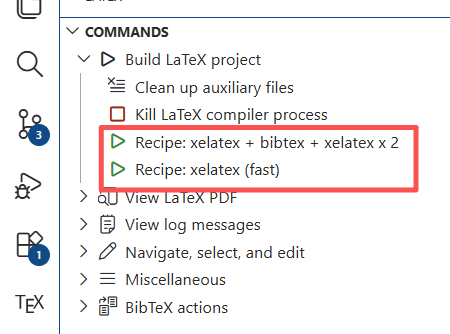
\includegraphics[scale=0.5]{figures/example.png}
    \caption{
        这里是个普通的标题
    }
    \label{fig:example}
\end{figure}

\begin{figure}[htb]
    \centering
    \begin{minipage}[t]{0.96\textwidth}
        \centering
        \begin{subfigure}[t]{0.47\textwidth}
            \centering
            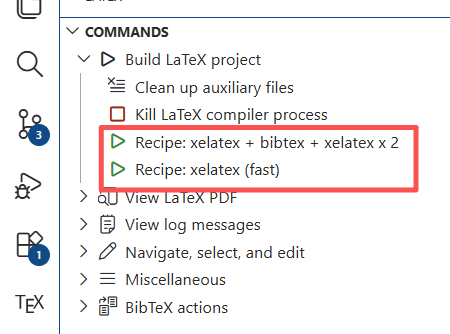
\includegraphics[scale=0.5]{figures/example.png}
            \caption{\label{subfig:example2-subfig1}}
        \end{subfigure}
        \begin{subfigure}[t]{0.47\textwidth}
            \centering
            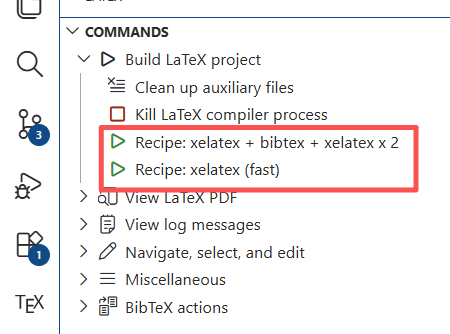
\includegraphics[scale=0.5]{figures/example.png}
            \caption{\label{subfig:example2-subfig2}}
        \end{subfigure}
    \end{minipage}
    \caption{这里是另一个普通的标题}
    \label{fig:example2}
\end{figure}


\cleardoublepage



%%=============================================================================%
%% 参考文献以及附录
%%-----------------------------------------------------------------------------%
\bibliographystyle{nputhesis-noslash}                       % 参考文献                                                  % 引用所有文献
\bibliography{ref/reference}                                    % 参考文献


\appendix
\chapter{一份说明 顺便测试英文标题 Title}

强烈不推荐英文标题！仅供测试，擅自使用后果自负。

\section{测试附录子标题}

这是一份附录，请放置一些独立的证明、源代码、或其他辅助资料。
\begin{equation}
    S = \pi r^2
\end{equation}

\cleardoublepage

%%=============================================================================%
%% 文档附页部分（致谢、参加科研情况、知识产权与原创性声明）
%%-----------------------------------------------------------------------------%
\backmatter                                                 % 文档附页部分
%%-----------------------------------------------------------------------------%
\begin{acknowledgements}                                    % 致谢开始
    感谢我的老师和我的朋友们……
\end{acknowledgements}                                      % 致谢结束
%%-----------------------------------------------------------------------------%
\begin{accomplishments}                                     % 参加科研情况开始
    [1] ...
\end{accomplishments}                                       % 参加科研情况结束
%%-----------------------------------------------------------------------------%

\makestatement                                              % 知识产权与原创性声明

\end{document}
